% Software
\specialsection{Software}{}{black}{white}

\begin{figure}
	\centering
	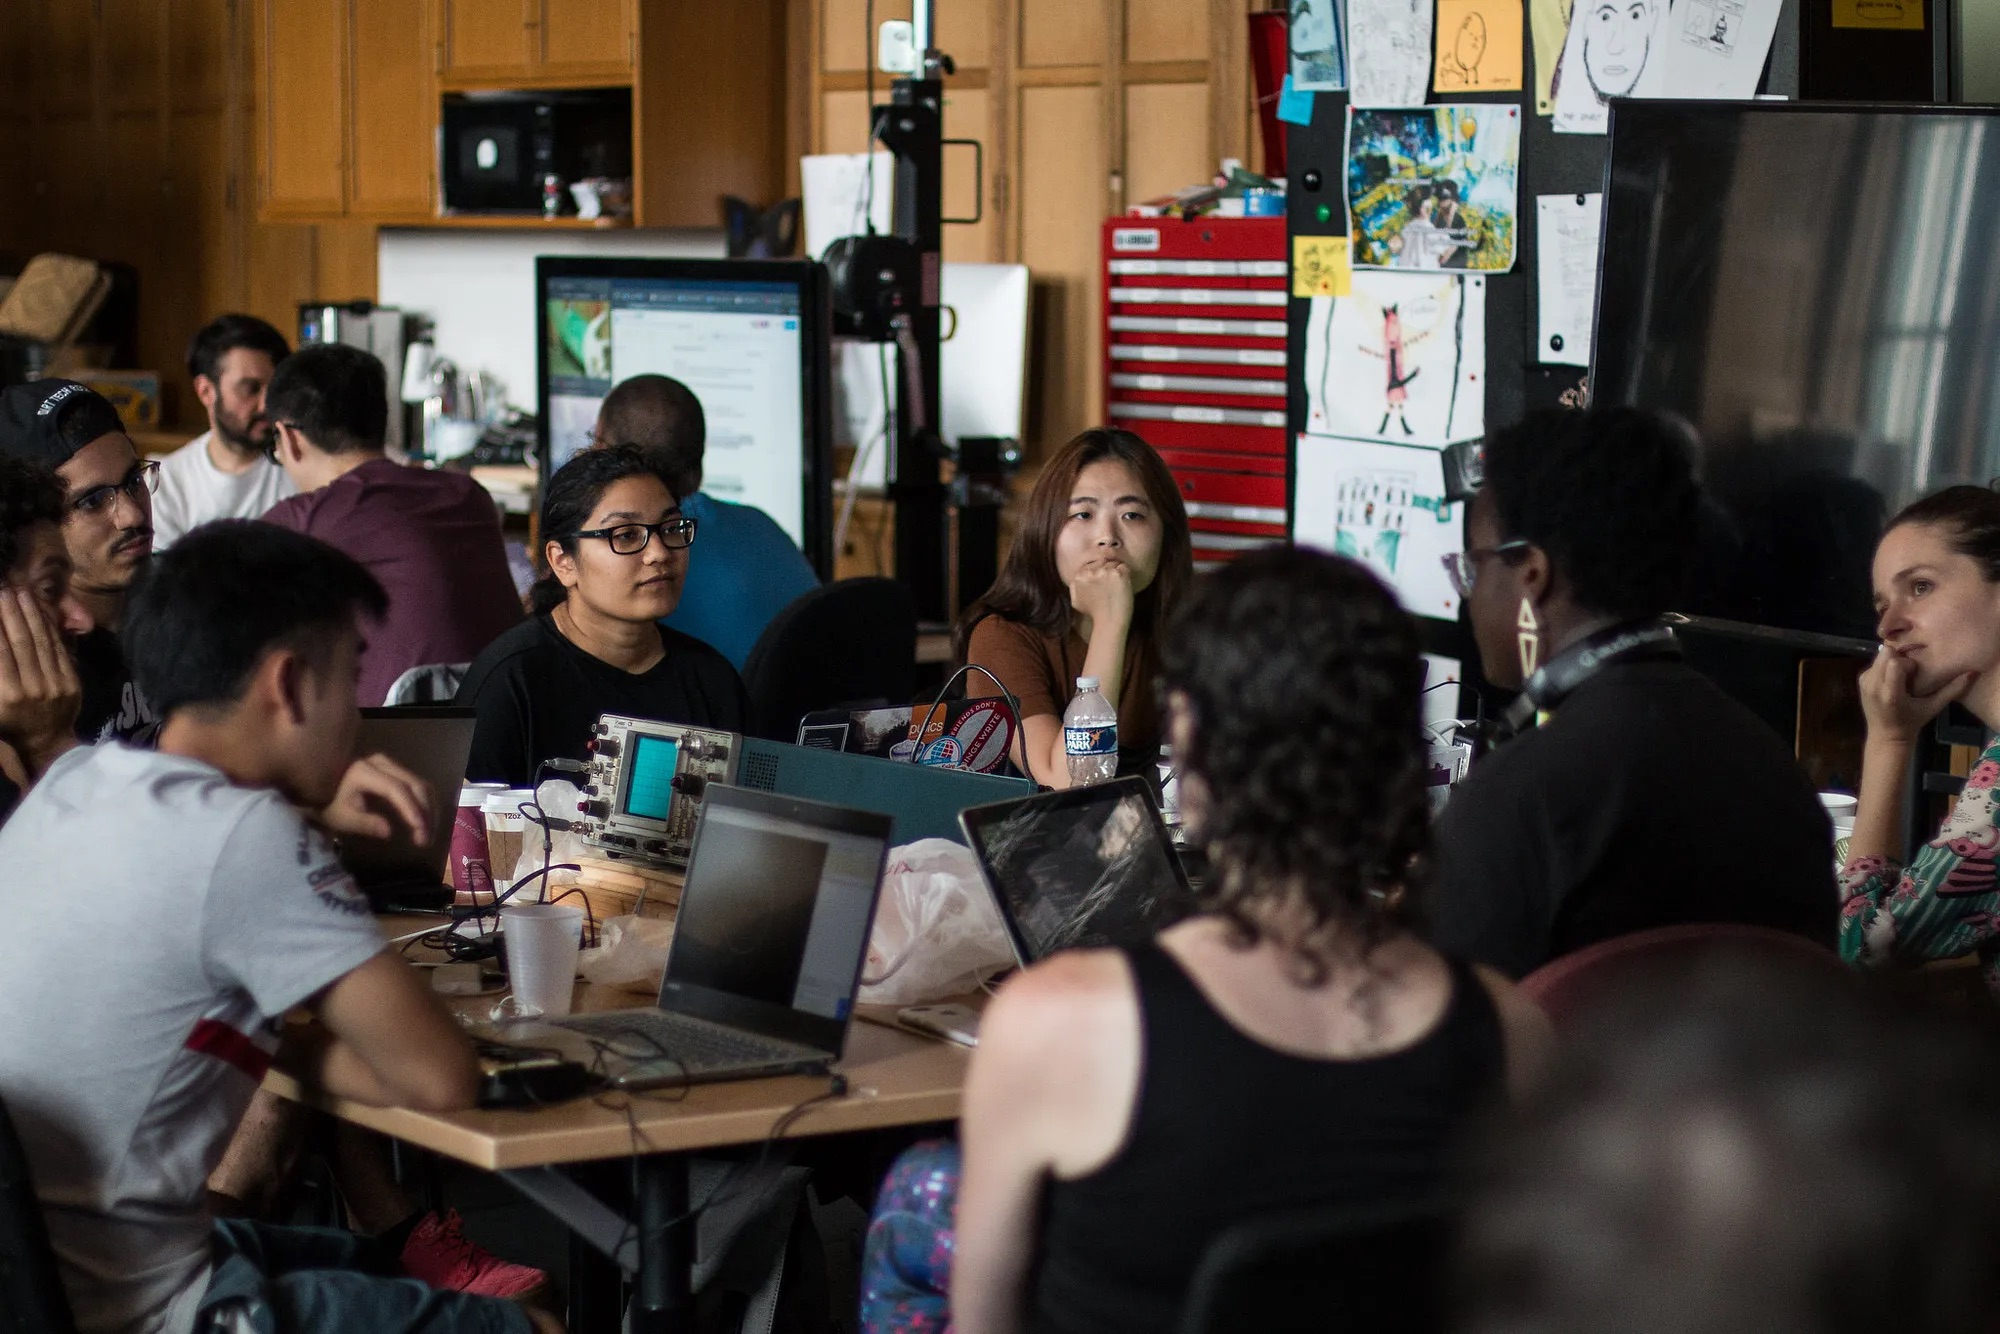
\includegraphics[width=\textwidth]{images/cathedral-or-bazaar.jpeg}
	\caption{Photograph from 2019 p5js Contributor Conference}
	\label{fig:p5ps-conference}
\end{figure}

\todo[inline]{Include image credit p5js project lead from zotero}

\subsection{Software Development Models}

The Processing project is commonly perceived as mainly the Integrated Development Environment (IDE) and its core components, which are crucial for basic operations. However, external libraries augmenting the system's capabilities are also essential to the ecosystem. 

This chapter delves into the distinctive mix of software development as applied to these two foundational aspects, from the core project, relying on a few dedicated contributors to the decentralized bazaar of library contributions and their interplay. Afterward, the mixed motivations of these different groups of code contributors are analyzed through a lens of technological, social, and economic factors. 

Eric S. Raymond's "The Cathedral and the Bazaar" \parencite{CathedralBazaarMusings2002a} identifies two open-source software development methodologies relevant to the processing project. 

The Cathedral model, exemplified by early GNU projects under Richard Stallman, is characterized by meticulous planning and centralized control \parencite{stallmanFreeSoftwareFree2002}. This model functions much like the construction of a cathedral, where a small group of experts crafts a complex, well‐organized structure over a long period, similar to the tiny number of contributors to the core processing project. 

In contrast, the Bazaar model, which gained prominence with the 
development of the Linux Kernel espouses a more decentralized approach. Spearheaded by Linus Torvalds, this model resembles a bazaar, where contributors from diverse backgrounds bring in their unique contributions, leading to rapid iterations and an evolving software landscape \parencite{TorvaldsLinuxKernelDevelopment1991}, reflective of the libraries ecosystem. 
These two models represent endpoints on a continuum, with many real-world projects, including Processing, displaying characteristics of both. 

While the Cathedral and Bazaar models provide a structural understanding of software development practices, exploring why individuals engage in these projects is equally essential. The sustainability of open‐source projects like Processing hinges on the continuous flow of software contributions. Without the active and sustained involvement of contributors, the long‐term viability of such projects is at risk. To gain a deeper understanding of what drives these contributions, we turn to the established taxonomy by Bonaccorsi et al. ~\ref{tab:taxonomy} \parencite{bonaccorsiComparingMotivationsIndividual2006} to facilitate comparison with other open-source projects.

This framework categorizes the motivations behind open‐source
contributions into Economic, Social, and Technological domains.

The following chapters analyze the dynamics and motivations of contributions to the core and libraries, respectively. The analysis combines quantitative data from software releases and version control systems with insights from interviews with key code contributors.

\begin{table}
    \begin{tabularx}{\textwidth}{l l} 
    \toprule
    Motivation area & Micro level \\
    \midrule
    Economic & Monetary rewards \\
     & Low opportunity costs \\
     & Gaining a reputation among peers \\
     & Gaining future career benefits \\
    \midrule
    Social & Fun to program (Loving to code) \\
     & Altruism (gift economy) \\
     & Sense of belonging to the community \\
     & Fight against proprietary software \\
    \midrule
    Technological & Learning \\
     & Contributions and feedback from the community \\
     & Working with a bleeding-edge technology \\
     & Scratching a personal itch \\
    \bottomrule
    \end{tabularx} 
    \label{tab:taxonomy}
    \caption{Taxonomy of Individual Programmers’ Motivations. Adapted from \parencite{bonaccorsiComparingMotivationsIndividual2006}}
\end{table}

\subsection{Core Contributions}
% What are core contributors
The core contributions here refer to the code that was integrated into the main chunk of the program delivered to people, specifically not to libraries or adjancent things. This not including only the bagel model.

% Data and methods
The quantitative data here was the releases data, reconstructed from log files, and the version control history commit history. Limitations: the releaseses are sometimes grouped together and sometimes information is missing, especially in the beginning, as it was done manually. The version control system was also changed a few times, so the logs might not be consistent. 
The commit logs within the Processing project's GitHub repository, while rich with data, do not provide a complete visualization of early contributions. In an interview with Ben Fry, it was elucidated that contributions from various lab members, including those from Simon Greenwold, were indeed substantial in the project's formative years. These contributions, although crucial, are not conspicuously traceable through the GitHub interface. Fry explains that due to the constraints of the version control systems like CVS and Subversion used at the time, he personally committed code from other contributors, ensuring their efforts were acknowledged in the commit logs, even if not directly attributed in the repository's graphical interface.
It is important to note that the data over represents Ben's contributions in the beginning, mainly because of the limitations of proper crediting and integration due to the version control systems (CVS and later subversion being used at the time)
While things were in CVS, I had to do the commits myself, but always noted where things came from in the commit history. It improved a little with Subversion and Google Code, but only by a little. GitHub was the first meaningful change where it really helped with the collaborative side of development. 
It is worth noting that the logistics of releasing software were more complex in the early 2000s than they are today. As can be seen in Figure~\ref{fig:processing-cd} of a mini CD from October 2002 illustrates, distributing software was not as straightforward as pushing updates to a Git repository.

% Data to interviews
Interviews were conducted with Ben Fry, the software engineering lead, Karsten Schmidt (toxi), code contributor and active member, and Simon Greenwold, core contributor and also member of the Aesthetics and Computation Group at MIT at the time. These people were selected here because they can be seen among the few contributors during the activity time of the Alpha Forum as can be seen on figure XXX. \todo[inline]{Mention code contributions of toxi and Simon Greenwold}

\changepapersize{305.3mm:210mm}
\customtag{largepage}

{
	\LARGE
	\noindent Frequency of Releases\par
	\vspace{0.2cm}
}

\begin{multicols}{3}
	\noindent
	\begin{minipage}{\columnwidth + \columnsep}
		\begin{tabular}{|r|l|}
			\hline
			Descriptive statistics & Time between releases \\
			\hline
			count                  & 60                    \\
			mean                   & 20 days 15:11         \\
			std                    & 47 days 00:10         \\
			min                    & 0 days 00:00          \\
			25\%                   & 1 days 00:00          \\
			50\%                   & 3 days 00:00          \\
			75\%                   & 26 days 18:00         \\
			max                    & 338 days 00:00        \\
			\hline
		\end{tabular}
		\captionof{table}{Release statistics}
		\label{tab:release-statistics}
	\end{minipage}
	\columnbreak
	\noindent
	\begin{minipage}{\columnwidth}
		\frame{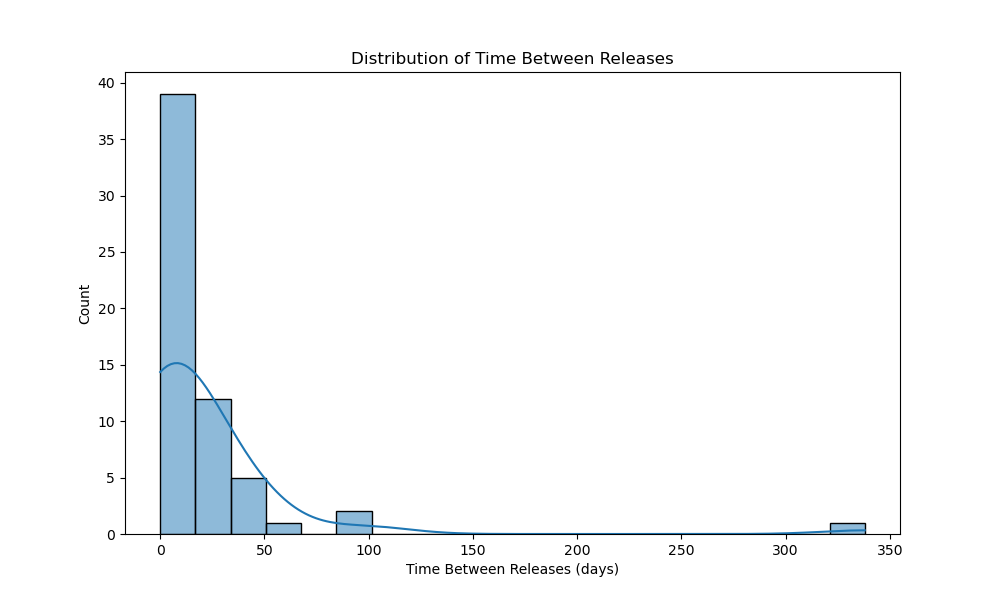
\includegraphics[width=\linewidth]{images/time_between_releases_histogram.png}}
		% \includegraphics[width=\linewidth]{graph2}
		\captionof{figure}{Graph that spans one column}
		\label{fig:releases-histogram}
	\end{minipage}
\end{multicols}

\begin{figure}[h!]
	\centering
	\frame{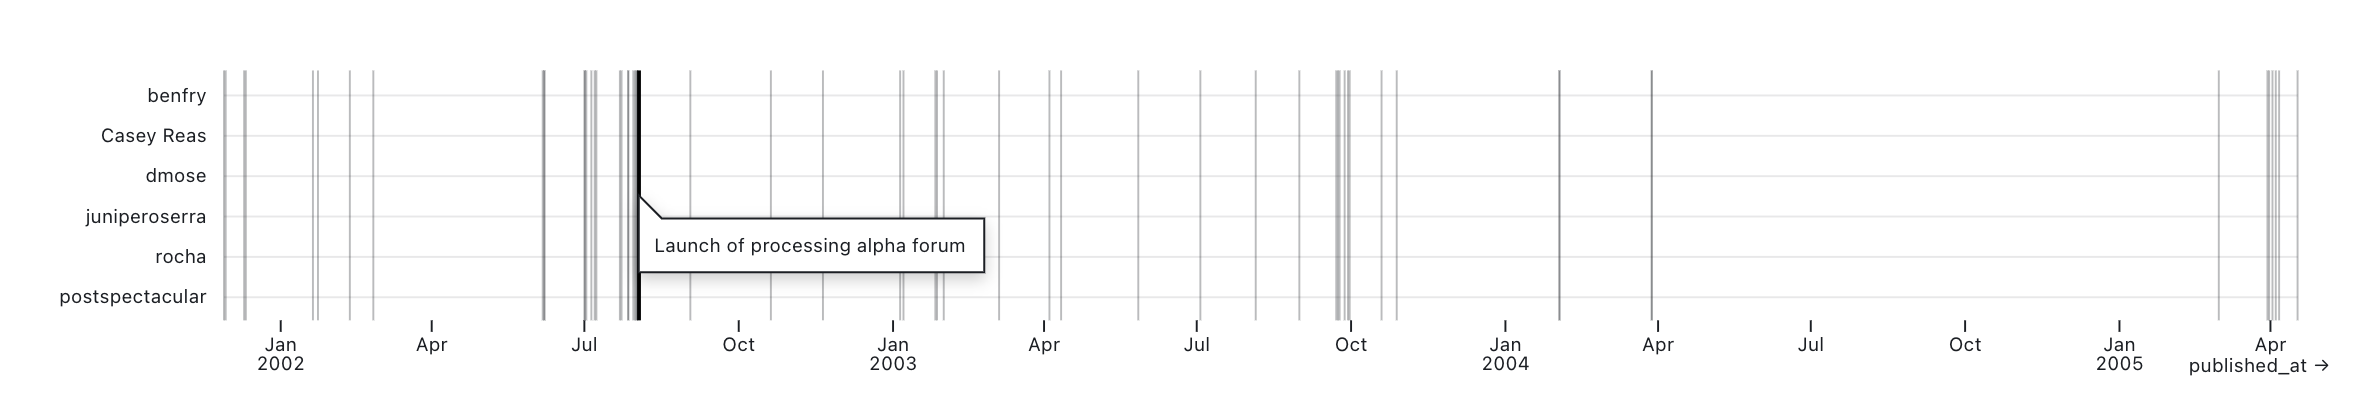
\includegraphics[width=1\textwidth]{images/releases-lines.png}}
	\caption{Time between releases}
	\label{fig:releases-lines}
\end{figure}

% \begin{figure}[h!] 
%   \centering
%   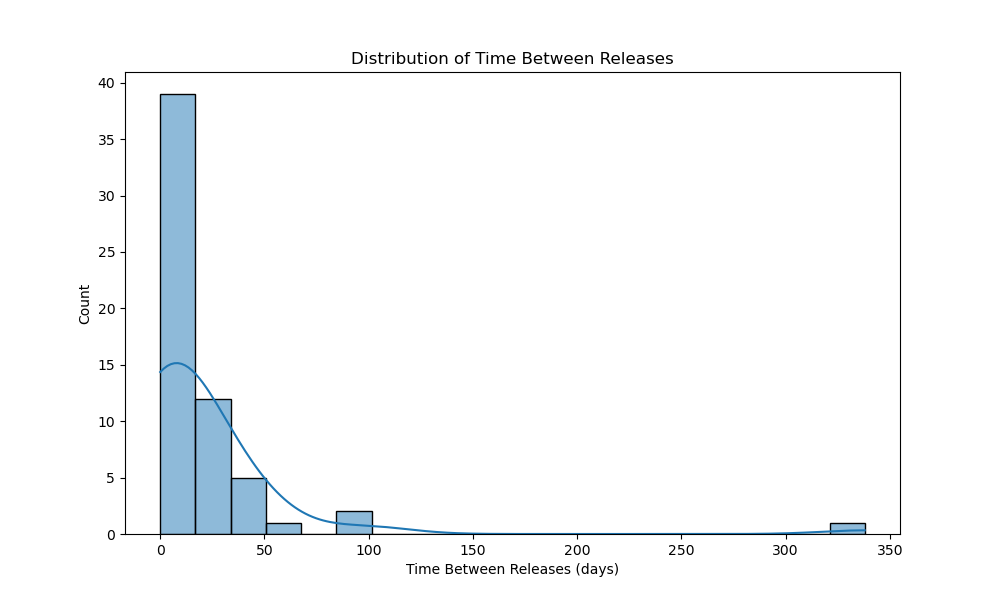
\includegraphics[width=0.9\textwidth]{images/time_between_releases_histogram.png} 
%   \caption{Time between releases histogram}
%   \label{fig:releases_frequency_histogram}
% \end{figure}

\begin{multicols}{3}
	\noindent
	The graphical representations depict a distinctive pattern of release clustering, a testament to the sporadic and intermittent nature of the project's development lifecycle. A notable surge can be observed leading up to pivotal milestones, such as the alpha forum's initial release, indicating a focused burst of activity during these critical junctures.
	\noindent
	The distribution of releases further accentuates the project's non-linear progress, with a marked increase in releases as key points approach, followed by periods of relative inactivity. This ebb and flow suggest that the development process is influenced by external factors or revolves around specific events, leading to a "feast or famine" scenario in terms of updates and improvements.
	\noindent
	Moreover, the extended intervals devoid of any releases could imply that the project advancement is perhaps a secondary or parallel endeavor for the contributors.
\end{multicols}

\defaultareasettings


\cleardoublepage
\changepapersize{305.3mm:210mm}
\customtag{largepage}

{
	\LARGE
	\noindent Version Control Statistics
}

\vfill

\noindent
	\begin{minipage}[t]{0.15\textwidth}
		\noindent
		\begin{figure}[H]
			\frame{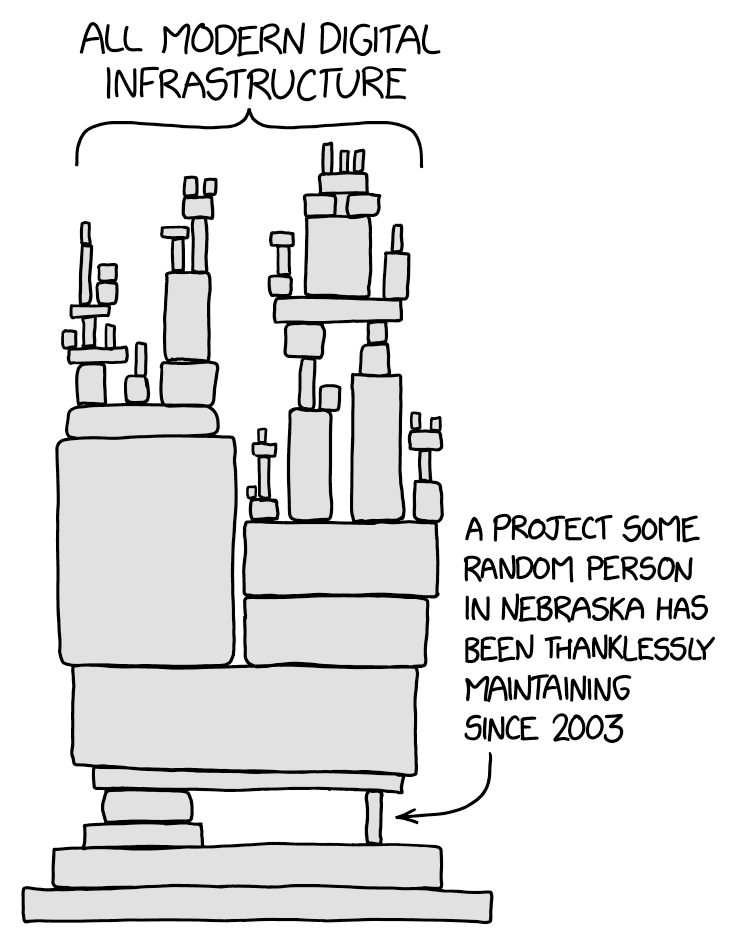
\includegraphics[width=\textwidth]{dependency.png}}
			\caption{Dependency comic}
			\label{fig:dependency_comic}
			% \small Source: \textit{XKCD}, \url{https://xkcd.com/2347/}, licensed under CC BY-NC 2.5.
		\end{figure}
	\end{minipage}
	\hspace{2mm}
	\begin{minipage}[t]{0.442\textwidth}
		\begin{figure}[H]
			\frame{\includesvg[pretex=\sffamily\fontsize{5.58pt}{8pt}\selectfont, width=\textwidth, keepaspectratio]{images/figure-top12-github.svg}}
			\caption[Top souce code contributors]{Top 12 source code contributors by number of commits in OCtober 2023}
			\label{fig:top12-github}
		\end{figure}
	\end{minipage}
\vspace{0.1cm}
\begin{figure}[H]
	\frame{\includesvg[pretex=\sffamily\fontsize{5.58pt}{8pt}\selectfont, width=1\textwidth, keepaspectratio]{images/processing-alpha-commits.svg}}
	\caption{Commits up to and including the Processing alpha forum}
	\label{fig:alpha-commits}
\end{figure}

\begin{multicols}{3}
	\noindent	
	The version control statistics portray a significant concentration of contributions by Ben Fry, indicating his pivotal role in maintaining the project across its timeline. The bar chart demonstrates Fry's preeminence through the sheer volume of his contributions relative to others. However, it's important to recognize that such visualizations do not fully encapsulate the breadth of contributions, especially in the project's nascent stages. Interviews suggest that many early contributions, made before the advent of sophisticated version control systems, remain unrepresented in these statistics. Thus, while the data underscores Fry's central involvement, it also omits a spectrum of foundational efforts that were integral to the project's initial development.
	\vfill\null
\end{multicols}

\defaultareasettings

% Initial Release: August 9 2001 -> Alpha Forum initial post: August 2 2002

In the development of the Processing project, Ben Fry's role as the main technical engineer was significant. This is underscored by the observations of his collaborators. Casey Reas emphasizes Fry's primary role: 'I think one thing that’s important to clarify is that Ben Fry, my collaborator, is the primary software engineer of the project' \parencite[p. 330]{conradGraphicDesignPostdigital2021}. Simon Greenwold further corroborates this, highlighting Fry's authoritative approach: 'He's maintaining strong control, like it's his code base. I think that's part of why it's great' (Greenwold, personal communication).

Completing the development of Bagel, the initial render engine, Ben Fry had established a robust code base a year before the debut of the processing alpha forum, prior to involving other contributors.

Fry discusses the early obstacles with MIT's Technology Licensing Office (TLO), particularly concerning intellectual property rights and the public release of the code. He details the extensive delays due to MIT, and more specifically the Media Lab, reevaluating their approach to open-source software, leading to an extended period of awaiting clearances.

Simon Greenwold underscores Processing's early adoption of an open-source model, a notable deviation in the context of Creativity Sustaining Toolkits (CST) for visual arts. He states, "Processing was notable in being open source early, ... probably unique in its class," thereby highlighting its pioneering role. In contrast, contemporaneous toolkits like Director or Flash were predominantly closed-source

Processing's development initially adhered to a centralized, cathedral-style model, characterized by structured, top-down control. The introduction of the alpha forum, however, marked a significant shift towards a decentralized, bazaar-style approach, encouraging community participation and collaborative code sharing.

This transition in Processing's development mirrors the early stages of other open-source projects like Linux, which also started with a solid foundation and evolved through community contributions. This shift to a more inclusive and collaborative model is a common trend in the development of open-source software.

The impact of this shift was evident in specific updates. The release notes from 27/05/2003 - rev 55, for instance, marked a turning point with the incorporation of code from external contributors, reflecting a move towards a community-driven development model. Following this, rev 56 further showcased the diversity of community involvement. It wasn't limited to code contributions; members engaged in various activities, including testing, providing feedback, and enhancing documentation. This broadened participation exemplified the multifaceted nature of the bazaar model, where contributions extend beyond programming to encompass various aspects of software development.

Building on this community-centric approach, the project adhered to Eric S. Raymond's principle: 'Treating your users as co-developers is your least-hassle route to rapid code improvement and effective debugging' \parencite[27]{raymondCathedralBazaar1999}. This ethos was crucial in Processing's evolution, particularly in the role of Ben Fry, who was integral in reviewing and integrating these diverse contributions, a strategy vital for the project's sustained success and functionality \parencite{Processing4CONTRIBUTINGMd}.

As the community's aspirations grew, a library system was introduced to accommodate the diversifying needs of the project, a topic explored in greater depth in the following chapter.

Eric S. Raymond's 'Release early, release often' philosophy further propelled Processing's vibrant development \parencite[28]{raymondCathedralBazaar1999}. This approach, which greatly benefited Linux, enabled rapid incorporation of contributions and fostered a responsive environment. The early phase of Processing, with 162 revisions prior to version 1 as shown in Figure~\ref{fig:releases-lines} and Table~\ref{tab:release-statistics}, was characterized by frequent updates, echoing Raymond's observation about Linux's development: 'In those early times (around 1991) it was not unknown for Linus Torvalds to release a new kernel more than once a day!' \parencite[28]{raymondCathedralBazaar1999}.

However, Processing's development was occasionally constrained by its nature as a side project. A comment from a revision in January 2003 highlights this: 'hopefully January 2003 will be a good month for p5, as I have a short bit of time to work on it [...] I hope to get a few revisions out this month so I can get back to my 'real' work.' This comment reveals Processing's status as a secondary commitment for its core contributors.

This aspect of Processing's development is detailed in a book titled 'Graphic design in the post-digital age: a survey of practices fueled by creative coding,' which notes that Processing began as a personal initiative, mainly developed during nights and weekends. The project's funding sources, including MIT's indirect support through Fry's graduate stipend and the Interaction Design Institute Ivrea (IDII)'s support through Reas's salary, further underscore its ancillary status \parencite[396]{conradGraphicDesignPostdigital2021}.

This part-time commitment likely impacted the level of engagement in the project. As Raymond puts it, regarding Linux: 'Linus was keeping his hacker/users constantly stimulated and rewarded—stimulated by the prospect of having an ego-satisfying piece of the action, rewarded by the sight of constant (even daily) improvement in their work' \parencite[28]{raymondCathedralBazaar1999}. In contrast, Processing's intermittent development schedule may have limited its potential for maximal engagement.

This engagement disparity becomes more evident when examining the contribution landscape within the Processing project, as depicted in Figure~\ref{fig:alpha-commits}. The figure highlights Ben Fry's central role, especially during the alpha forum phase. Notably, only six individuals, including Fry, actively contributed code to the repository, a stark contrast to the more than 1000 individuals engaged in forum discussions. Such a scenario suggests that Fry's involvement was not just central but potentially overshadowing, limiting the scope for broader community contributions. This aspect is particularly crucial given the acknowledged limitations of version control systems in fully capturing the nuances of individual contributions.

Fry's predominant role in Processing raises critical concerns about the project's resilience and sustainability, as observed in many open-source initiatives. Over the past two decades, his extensive contributions have been indispensable. Yet, they also introduce a high-risk factor known as the "bus factor" \parencite{BusFactor2023}, reflecting the project's vulnerability due to its heavy reliance on a few key individuals. This phenomenon, while common across open-source projects and often humorously depicted in popular culture \parencite{munroeDependency2020}, poses a significant challenge to the long-term health of Processing.

The discrepancy between the small cadre of code contributors and the expansive forum community is further underscored in subsequent visualizations (see Figures~\ref{fig:top12-github} and \ref{fig:dependency_comic}). This imbalance not only reflects the concentrated responsibility on a handful of developers, prominently featuring Fry, but also amplifies the risks associated with the bus factor. Addressing this disparity is vital for the sustainable future of the Processing project, necessitating a deeper exploration of strategies to diversify and expand its development base.

The contribution landscape within the Processing project, as vividly illustrated in Figure~\ref{fig:alpha-commits}, further highlights Fry's central role. During the alpha forum phase, only six individuals actively contributed code to the repository, contrasting sharply with the over 1000 individuals engaged in forum discussions. As previously discussed, it is important to bear in mind the limitations of the version control system's depiction of contributions.

The \textit{Processing} project illuminates a crucial challenge often faced by open source communities: the dependency on key contributors. In the case of Processing, Ben Fry's central role over the past two decades raises concerns about the project's resilience and sustainability. His substantial contributions create a high-risk situation termed the "bus factor" \parencite{BusFactor2023}, which indicates how vulnerable a project becomes when overly reliant on a single or a small number of contributors. This vulnerability is not unique to Processing, as such dependency models are commonly observed across open source projects, often humorously discussed in popular culture \parencite{munroeDependency2020}.

This discrepancy between the number of code contributors and forum participants is indeed profound, as corroborated by the subsequent visualizations ~\ref{fig:top12-github} and comic anecdotes ~\ref{fig:dependency_comic}. The limited number of contributors to the codebase and the concentrated responsibility on a few individuals amplify the bus factor risk, an issue that warrants deeper investigation and consideration for the long-term health of the project.

% Motivations according to the taxonomy
Transitioning from the observed discrepancy between the wide forum engagement and the limited core code contributors, it is pivotal to contextualize the commitment of these few key individuals within a structured framework. The taxonomy by Bonaccorsi et al.~\cite{bonaccorsiComparingMotivationsIndividual2006} provides a valuable lens through which to examine their motivations. This taxonomy categorizes the motivations into Economic, Social, and Technological factors, each offering a distinct perspective on the individual's involvement.

Ben Fry’s technological motivation for developing Processing is deeply rooted in his personal experience with the cumbersome nature of existing tools for computational design. His aim was to create a platform that could sidestep these complexities, thus “scratching his own itch” and aid in teaching:

\begin{quote}
	“As researchers, all those extra steps just got in the way: we already knew how to do those things, and it just made the process tedious. So with Processing, we wanted to get closer to just having things show up and work.” 
\end{quote}

This technological motivation is also echoed by Karsten Schmidt, whose initial involvement was propelled by the technological potential and the the opportunities within the young Processing project:

\begin{quote}
"The project was still young, there was a lot of stuff to do ... So I was not really a Processing user in the beginning. I became a user as I was contributing code to the actual tool." 
\end{quote}

The economic incentives for engaging with Processing were not clear, Simon Greenwold’s statement highlights the absence of monetary gain and the low economic competition in the field:
\begin{quote}
	“There's no money in it. So who's going to come challenge it, right?” 
\end{quote}
	
Yet, despite the lack of financial motivation, Processing found significant traction in educational settings, where the alternatives left much to be desired. Greenwold’s assessment of the other tools available at the time underlines this point:
	
\begin{quote}
"They were terrible. Just terrible. Yeah, Flash the director and Flash weren't the same yet. They came together and then both died." 
\end{quote}

The role of Processing in education is further substantiated by visual evidence, as illustrated in the community survey results conducted in 2016, which underscore its widespread adoption as a teaching tool.
\todo[inline]{Add ref to community survey}

The social aspect of Fry’s motivations cannot be understated. His commitment to teaching and sharing knowledge, particularly with individuals who may not have coding expertise, signifies a strong social incentive that aligns with the open-source ethos of knowledge dissemination:

\begin{quote}
	"One of the most important things about the community for me personally is the motivation that comes from seeing really talented people use tools like this. That's realy exciting and makes me want to work harder."
\end{quote}
\begin{quote}
“I learned to code at a very young age because other people shared their code... Their willingness to share, or even answer questions of a 9- or 10- or 12-year-old was a pretty incredible gift, and had a huge impact.” 
\end{quote}

Fry’s dedication to education and community engagement is a testament to the social motivations that are central to the Processing project. This commitment has not only fostered a supportive community but also helped proliferate computational design skills among a broader audience, further amplifying the project's impact.

In sum, the core contributors to Processing, already posessing strong technical skills, have been driven by a confluence of motivations. Technologically, they aimed to create a tool that would overcome the limitations of existing software. Economically, while there was no direct financial incentive, the educational adoption of Processing has led to an increase in its use and, indirectly, its importance in the computational design landscape. Socially, the emphasis on teaching and sharing knowledge has been a cornerstone of the project’s philosophy, ensuring that Processing remains an accessible and community-focused platform.

\begin{figure}[h!]
	\centering
	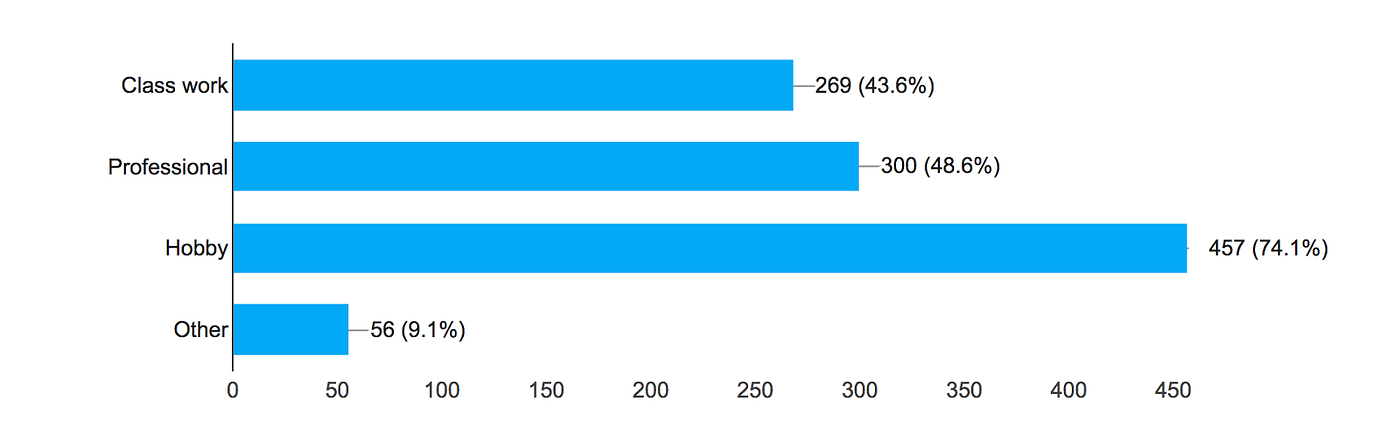
\includegraphics[width=\textwidth]{images/community-survey.png}
	\caption{Processing 2016 community survey result \parencite{2016CommunitySurvey}}
	\label{fig:community_survey}
\end{figure}

\subsection{An ecosytem of libraries}
The integration of libraries marked a significant turning point in the Processing ecosystem. These additions expanded the core platform's capabilities, thus drawing a wider array of users and contributors. In the Processing community, libraries have been indispensable, acting as fundamental components that not only enhance the platform’s functionality but also encourage inventive exploration.

This evolution in development philosophy is captured through the insights of Casey Reas, a co-founder of Processing. Reflecting on the initial phases of Processing's development, Reas observed, "One of the important early decisions was to make what we call 'libraries.' Ben [Fry] and I realized that we were in a bottleneck and getting in the way of how people wanted to expand and extend Processing" \parencite[329]{conradGraphicDesignPostdigital2021}. This statement underscores the pivotal shift towards an approach that embraced openness and collaborative progress in the development process.

The development and integration of libraries within the Processing ecosystem primarily exemplify the bazaar model of software development, with a nod to the modularity characteristic of the GNU model. This is particularly evident in how some libraries evolved into core components of Processing.

A notable example is the development of the OpenGL renderer by Andrés Colubri. This library, initially developed independently to enhance Processing's performance, was later integrated into the main software following its widespread acceptance within the community. This integration process is a classic example of the bazaar model, where development is open, collaborative, and evolutionary, driven by the diverse needs and contributions of the user base. \parencite{Processing4CONTRIBUTINGMd}

While the modularity and individual contributions in this process bear some resemblance to the GNU model, it is important to note that Processing's approach is more reflective of the dynamic and decentralized nature of the bazaar model. The bazaar model emphasizes open collaboration and iterative development, which is more aligned with the community-driven development culture seen in Processing.

% Data analysis
Utilizing publicly available data from the Processing website archive, I successfully reconstructed the release history of various libraries between October 2011 and June 2014. This period reflects active development and frequent releases across multiple library categories, as illustrated in Figure~\ref*{figure:libraries}. As a result of the absence of earlier data, it led to a somewhat arbitrary choice of interview subjects from this time period. Consequently, the insights obtained may not fully represent the experiences within the Processing community at it's beginning. Despite these limitations, the interviews provided valuable qualitative insights into the motivations and contributions of library developers. 

\todo[inline]{Include graphic of specific libraries}



When analyzing interviews guided by Bonaccorsi et al.'s taxonomy, it becomes clear that technological innovation and community engagement were the primary driving forces behind the contributors. For instance, Karsten Schmidt's experiences reflect a strong technological motivation. He aimed to push the limits of computational design's expressive potential and, as a result, was compelled to create tools such as toxiclibs. This library aligned more closely with his vision than other frameworks, such as Flash or Director, which constrained creative expression within predefined roles and stage-based metaphors like directors, actors, and scripts. In his words, "I really wanted something new, the way I can be more expressive with the actual computational side, the algorithm side."

Similarly, Andreas Schlegel's development of ControlP5 was driven by a practical need in his projects. He sought a tool that could provide a more intuitive and effective way of managing user interfaces within Processing. Schlegel's creation of ControlP5 can be seen as 'scratching his own itch', addressing personal challenges that benefit the wider community, as he noted: "ControlP5 started as a need for sliders and buttons to control the visuals I was working on."

Marxer emphasized the collective effort and the shared sense of purpose among diverse individuals involved in open-source projects. He pointed out that these collaborative environments provide a platform for individuals from various backgrounds to learn from each other, contribute to a larger cause, and collectively advance the field. The social dynamics of open-source projects are crucial, as Marxer noted: "So it's a sense of community. I think, in a sense, of working together as a society."

According to Schlegel, his first library, oscP5, resulted from his final year project in his master's in media arts and technology, which focused on designing a computer network for artistic applications. Initially, he did not intend to write it for the community, but that came as an afterthought. Similarly, Marxer reflected that Geomerative was initially a technological tool to "do letters that were joined by the serifs," but it ended up being a whole project in generative typography.

As contributors like Schmidt and Schlegel delved deeper into the technology, they also became integral members of a burgeoning community. The collaborative ethos of the Processing community is evident in Marxer's statement: "yeah, the goal is that all the work you do, nobody else should go through that and do it." He was a DIY enthusiast, and he enjoyed seeing how things could be done. 

Schmidt also mentions that "open source was essentially amateur culture... there are labors of love for most people; it's what's done in their spare time or what comes out from some interesting work projects, what people want to share." Although not the primary draw, economic factors emerge in the narrative, albeit as a secondary consideration. Schmidt's indirect financial benefits from his open-source work underline this point: "in other times, I have indirectly made a living through my open-source work, but not directly from it." Schlegel's experience similarly reveals that while economic gain was not the goal, the recognition and opportunities that arose from his contributions had positive professional implications.

The interplay between these motivations underscores the complexity of open-source software development. The contributors are often initially attracted by the technological challenges. As they immerse themselves in the work, the community aspect becomes more significant, providing a supportive network for sharing and growth. This dynamic appears to be particularly relevant at the beginning of a project when the necessary tools and infrastructure have not yet been built out.


\cleardoublepage
\changepapersize{305.3mm:210mm}
\customtag{largepage}

\thispagestyle{empty}
\begingroup
\raggedright 
\vspace*{\stretch{1}}
\section*{Library Releases} 
\fontsize{12pt}{14pt}\selectfont
\vspace*{\stretch{1}}
\endgroup

\newpage
\customtag{largepage}

% {
% 	\LARGE
% 	\noindent Library Releases
% }

\begin{figure}[H]
	\includesvg[pretex=\sffamily\fontsize{5.58pt}{8pt}\selectfont, width=1\textwidth, keepaspectratio]{images/figure-libraries.svg}
	\vspace{3pt}
	\caption{Distribution of Libraries in the Processing Project}
	\label{figure:libraries}
\end{figure}

\begin{multicols}{3}
	\todo[inline]{Shorten this explanation, or move some parts elsewhere}
	\noindent
	This graph illustrates the distribution of Processing library releases over a period from January 2012 to April 2014. Each dot on the graph signifies a release event for a library in various categories such as 3D, Animation, and GUI. The process of releasing these libraries was manual, requiring approval on the Processing website before they became available for update. This artisanal method meant that only the latest versions of the libraries were accessible, without an option to retrieve previous iterations.
	\noindent
	The data for this graph was meticulously reconstructed using a 'git blame' operation on the data folder containing links to these libraries. It's worth noting that this data may not fully represent the entirety of the Processing library space. The reconstruction is based on a single version of the website's data, lacking a comprehensive historical record that could have been obtained from multiple website versions. Thus, while the graph provides valuable insights into the release patterns and activity within the Processing community, it comes with the caveat of being an incomplete representation due to the availability of only one snapshot of the website data.
	\noindent
	 Despite the limitations in data scope, it reflects a significant portion of the community's contributions and the evolution of library offerings during the specified timeframe.
\end{multicols}
\defaultareasettings



he academic and professional environments of library contributors like Ricard Marxer, Andreas Schlegel, and Simon Greenwold in the Processing community indeed present a stark contrast to the experiences of those primarily active in forums, such as Ariel Malka (arielm) and Jacob Schwartz (benelek).
Ricard Marxer's discovery of Processing during his master's studies in digital art around 2004-2005, set in a context that bridged programming and digital art, fostered an ideal environment for his library development. Unlike forum-centric users, Marxer's engagement with the Processing community was marked more by his technical contributions than by active forum participation. His self-taught background in computing and his focus on maintaining his library between 2002-2010, as opposed to seeking peer interaction on forums, underscores a different path within the community​​​​.

